\documentclass[../problems.tex]{subfiles}

\graphicspath{{../images/}}

\begin{document}
\section{Energy}
\barh

\paragraph{4.2}
From the origin $O$ to point $P = (1,1)$ a two dimensional force $\vb{F} = (x^2, 2xy)$ 
moves a point along three paths where the work done by the force is 
\begin{equation*}
    W = \int_O^P \vb{F} \cdot \dd{\vb{r}} = \int_O^P F_x \dd{x} + F_y \dd{y}
\end{equation*}
(a) Splitting the path into two parts $O \to Q=(1,0)$ and $Q \to P$, we have two integrals
\begin{align*}
    W &= \int_O^Q F_x \dd{x} + \int_Q^P F_y \dd{y}
\end{align*}
where the first integral accounts for just the $x$ component of force $F_x = x^2$ and the second
integral accounts for just the $y$ component of force when $x=1$; $F_y = 2(1)y$. Thus
\begin{align*}
    W = \int_0^1 x^2 \dd{x} + \int_0^1 2y \dd{y} = \frac{4}{3}
\end{align*}

(b) The path follows the parabola $y=x^2$ from $O \to P$. From $\dd{y} = 2x \dd{x}$ the integral
can be rewritten in terms of just $x$
\begin{align*}
    W = \int_0^1 x^2 \dd{x} + \int_0^1 2x (x^2) \dd{y} 
    = \frac{1}{3} + \int_0^1 4x^4 \dd{x} = \frac{17}{15}
\end{align*}

(c) Path follows the parametric curve $x=t^3$ and $y=t^2$ where the differentials are:
$dx = 3t^2 \dd{t}$ and $dy = 2t \dd{t}$. Thus the work done on the path is
\begin{align*}
    W = \int_0^1 (t^6) (3t^2 \dd{t}) + \int_0^1 (2t^3) (2t \dd{t}) 
    = \frac{1}{3} + \frac{4}{5} = \frac{19}{15}
\end{align*}

\paragraph{4.3}
Same as Problem 4.2 but with a force $\vb{F} = (-y,x)$ and three different paths from $P = (1,0) \to
Q = (0,1)$.

(a) This path follows a straight line $y = 0$ from $P \to O$ and then $x = 0$ from $O \to Q$. Thus 
the work done is 
\begin{align*}
    W = \int_P^O F_x \dd{x} + \int_O^Q F_y \dd{y} = 0
\end{align*}

(b) A straight line from $P \to Q$ is given by $y = -x + 1$ and the differential $dy = -dx$. Thus
the work done is
\begin{align*}
    W = \int_P^Q F_x \dd{x} + F_y \dd{y} 
    = \int_1^0 (-(-x+1)) \dd{x} + (x) (-\dd{x}) = \int_1^0 -1 \dd{x} = 1
\end{align*}

(c) The path of a quarter circle centered on the origin in polar coordinates is given by
\begin{align*}
    x = r \cos \phi \qquad y = r \sin \phi
\end{align*}
where $r=1$, $\phi = 0 \to \pi/2$ and the differentials are
\begin{align*}
    dx = \cos \phi d{r} - r \sin \phi \dd{\phi} = - \sin \phi \dd{\phi} \qquad
    dy = \sin \phi d{r} + r \cos \phi \dd{\phi} = \cos \phi \dd{\phi}
\end{align*}
Thus the work done is
\begin{align*}
    W = \int_P^Q F_x \dd{x} + F_y \dd{y} 
    = \int_0^{\pi/2} (-\sin \phi) (-\sin \phi \dd{\phi}) + (\cos \phi) (\cos \phi \dd{\phi})
    = \int_0^{\pi/2} \dd\phi = \frac{\pi}{2}
\end{align*}

\paragraph{4.5}
(a) Given the force of gravity $\vb{F} = -mg \vu{y}$ and vertical height from 1 to 2 $h = y_2 - y_1$
, the work done by gravity is 
\begin{align*}
    W_{g}(1 \to 2) = \int_1^2 \vb{F} \cdot \dd{r} = \int_0^h -mg \dd{y} = -mgh
\end{align*}
Since the force $\vb{F}$ depends only on position and the work done by is independent of the path
taken, the force is conservative.

(b) The gravitational potential energy of the particle is 
\begin{align*}
    U_g(\vb{r}) = - W_g(0 \to \vb{r}) = - \int_0^{\vb{r}} \vb{F} \cdot \dd{\vb{r}} 
    = - \int_0^{\vb{r}} -mg \dd{y} = mgy
\end{align*}
where $\vb{r} = y\vu{y}$ is the position vector of the particle.

\paragraph{4.7}
(a) Given the gravitational force has magnitude $F_y = -m\gamma y^2$, the work done by gravity is
\begin{align*}
    W = \int_1^2 F_y \dd{y} = \int_1^2 m\gamma y^2 \dd{y} = \frac{1}{3} m\gamma (y_2^3-y_1^3)
\end{align*}
The gravity is still conservative since the work done by gravity is independent of the path taken
and the force depends only on position. Hence, the corresponding potential energy is
\begin{equation*}
    U_g(\vb{r}) = - W(0 \to \vb{r}) = - \int_0^{y} F_y \cdot \dd{y'} = \frac{1}{3} m\gamma y^3
\end{equation*}

(b)
\begin{figure}[ht]
    \centering
    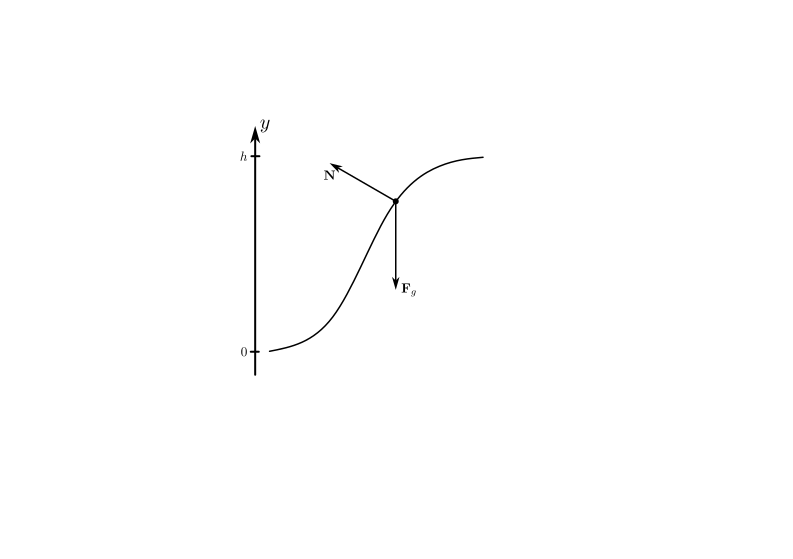
\includegraphics[scale=0.7]{../images/fig4_7.png}
    \caption{A threaded bead on a wire with two forces acting on it; The force of gravity $\vb{F}_g$
    is conservative and the normal force $\vb{N}$ is non-conservative.}
    \label{fig:4_7}
\end{figure}

(c) The bead is initially released from rest at a height $h$. From conservation of energy:
\begin{align}
    E_i &= E_f \\
    \frac{1}{3} m\gamma h^3 &= \frac{1}{2} m v^2 \\
    v &= \sqrt{\frac{2}{3} \gamma h^3}
\end{align}
where $v$ is the speed of the bead at the bottom of the wire.

\paragraph{4.9}
(a) Assuming the force of a one-dimensional spring $F = -kx$ is conservative, potential energy is
\begin{align*}
    U(x) = - \int_0^x F \dd{x'} = \frac{1}{2} kx^2  
\end{align*}
where $x$ is the displacement of the spring from its equilibrium position.

(b) From Newton's second law, the new equilibrium position $x_o$ is found when the spring force and
gravity are equal.
\begin{align*}
    0 = F + F_{g} = -kx_o + m g \implies x_o = \frac{mg}{k}
\end{align*}
When $y = 0$,  $U = 0$. Thus the potential energy is zero at position $x = x_o$:
\begin{align*}
    U(x_o) = \frac{1}{2} k(x_o)^2 - mg(x_o) = 0
\end{align*}
The total potential energy of the system at position $x = y + x_o$ is
\begin{align*}
    U(x) &= U_{sp} + U_{g} = \frac{1}{2} k(y+x_o)^2 - mg(y+x_o) \\
    &= \frac{1}{2} ky^2 + kyx_o - mgy + \frac{1}{2} kx_o^2 - mgx_o
\end{align*}
Since $kyx_o - mgy = 0$ and the last two terms are the potential energy at the new equilibrium
$U(x_o) = 0$, the total potential energy is $U(x) = \frac{1}{2} ky^2$.

\paragraph{4.11}
Finding the partial derivatives of the functions with constants $a,b,c$:

(a) $f(x,y,z) = ax^2 + bxy + cy^2$:
\begin{align*}
    \pdv{f}{x} &= 2ax + by \qquad \pdv{f}{y} = bx + 2cy \qquad \pdv{f}{z} = 0
\end{align*}

(b) $g(x,y,z) = \sin(axyz^2)$:
\begin{align*}
    \pdv{g}{x} &= ayz^2 \cos(axyz^2) \qquad \pdv{g}{y} = axz^2 \cos(axyz^2) 
    \qquad \pdv{g}{z} = 2axyz \cos(axyz^2)
\end{align*}

(c) $h(x,y,z) = ar$ where $r = \sqrt{x^2 + y^2 + z^2}$:
Since 
\begin{equation*}
    \pdv{r}{x_i} = \frac{x_i}{r}
\end{equation*}
The partial derivatives of $h$ are
\begin{align*}
    \pdv{h}{x} &= \frac{ax}{r} \qquad \pdv{h}{y} = \frac{ay}{r} \qquad \pdv{h}{z} = \frac{az}{r}
\end{align*}

\paragraph{4.13}
\end{document}